
\section{Motivation}

\begin{figure}[ht]
  \centering{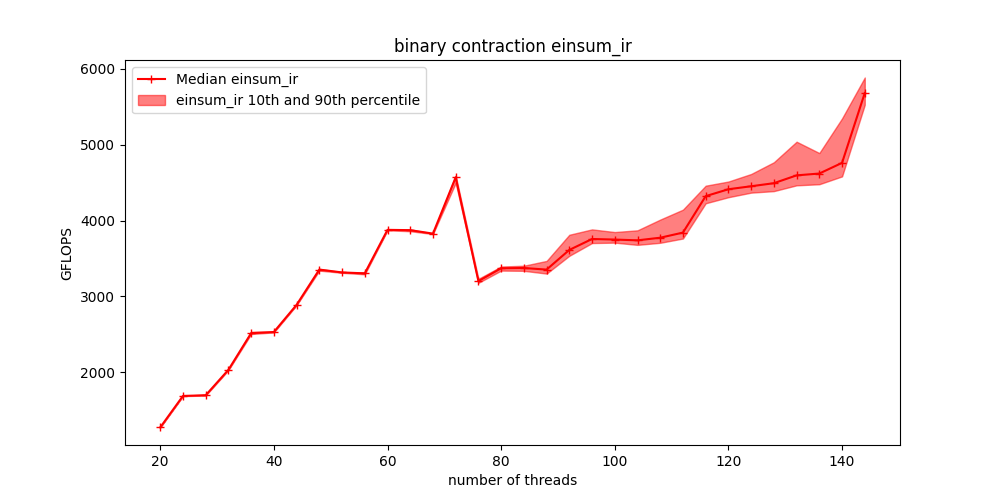
\includegraphics[width=0.95\textwidth]{gflops_threads.png}}
  \caption{
    Performance of einsum\_ir on an Nvidia Grace CPU Superchip.
    Grace consists of two 72-core CPUs connected via NVLink.
    The contraction used is $m_0c_0k_0k_1m_1, n_0c_0k_0n_0n_1 \rightarrow m_0n_0c_0n_1m_1$ with $|c_0|=2$, $|m_0|=|n_0|=|k_0|$ and $|m_1|=|n_1|=|k_1|=70$.
    JIT compilation times of \texttt{einsum\_ir} are included in the measurement.
    }
  \label{fig:perf_threads}
\end{figure}

\texttt{einsum\_ir} already implements shared memory parallelization with OpenMP\cite{openMP}, so it can already exploit all CPU cores on a single NUMA domain.
But as shown in Figure \ref{fig:perf_threads} the performance breaks down as soon as more than one NUMA domain is used.
Even using all threads on Grace improves the performance by merely 24\% over only using one socket.
The goal of this thesis is to improve this scaling behavior across NUMA domains.

To achieve this goal we look at four distributed memory algorithms.
Before going over these algorithms in detail we should look at how other applications parallelize similar workloads.
Parallelizing tensor operations is essential to machine learning, so we can take lessons from that field.
The most popular practices to parallelize machine learning workloads are data, tensor and pipeline parallelism \cite{megatronLM}.
Data parallelism is specific to the training phase of machine learning models, where the weights of a model get updated in parallel.
We do not want to restrict ourselves to only AI training workloads, so this type is not applicable.
That leaves tensor and pipeline parallelism.
Tensor parallelism is generally favored when scaling across a single node \cite{megatronLM}, while pipeline parallelism performs better when scaling across nodes.
Since our motivation stems from accelerating \texttt{einsum\_ir} on a single execution node primarily, I decided to pursue tensor parallelism.


\section{Master-Worker Algorithm}

As our first algorithm we think of a master-worker architecture to improve performance across NUMA domains.
Since the main hardware target were dual socket servers, like the Nvidia Grace CPU Superchip, we restrict our algorithm to two processes.
This also trivially ensures that the communication is balanced between all processes.
The basic premise of this algorithm is treating the worker as a matrix accelerator where you send parts of the input matrix to and receive the corresponding parts of the output matrix from.
Since both NUMA domains should ideally be equally fast we cut all tensor across one c-dimension $c_0$ into $|c_0|$ chunks, with the master working on the first $\left \lceil{\frac{|c_0|}{2}}\right \rceil $ chunks together as one big contraction and send  the remaining  $\left \lfloor{\frac{|c_0|}{2}}\right \rfloor$ chunks to the worker to process them in parallel to the master process.
To enable the overlap of communicating with the other process and computing the chunks, each process uses one of its thread exclusively as communication thread.
This thread is solely responsible for communicating the input chunks from the master to the worker and the output chunks from the worker back to the master.

From the perspective of the master thread the communication and compute threads only have to synchronize at the end of the contraction, waiting for the other to finish.
The worker's compute threads however have to wait until their input data is fully assembled before they can start working.
To minimize the waiting times the computation and communication goes as follows, with $A_i$, $B_i$ and $C_i$ each being the $i$-th chunk contracted on the worker:

\begin{center}
  \begin{tabular}{ |c|c| } 
  \hline
  compute threads & communication thread\\
  \hline
   & \texttt{receive} $A_1$ and $B_1$\\
  \hline
  $A_1,B_1 \rightarrow C_1$ & \texttt{receive} $A_2$ and $B_2$\\
  \hline
  $A_2,B_2 \rightarrow C_2$ & \texttt{receive} $A_3$ and $B_3$\\
  & \texttt{send} $C_1$\\
  \hline
  \multicolumn{2}{|c|}{\dots}\\
  \hline
  $A_k,B_k \rightarrow C_k$ & \texttt{receive} $A_{k+1}$ and $B_{k+1}$\\
  & \texttt{send} $C_{k-1}$\\
  \hline
  \multicolumn{2}{|c|}{\dots}\\
  \hline
  $A_n,B_n \rightarrow C_n$ & \texttt{send} $C_{n-1}$\\
  \hline
  & \texttt{send} $C_n$\\
  \hline
\end{tabular}
\end{center}

The communication thread of the master matches each \texttt{receive} of the worker with a \texttt{send} and each \texttt{send} of the worker with a \texttt{receive}.
The workers compute threads have to synchronize with its communication thread after each row.
To minimize the initial memory allocation on the worker it only has 2 buffers for $A$, $B$ and $C$ chunks respectively.
This is possible since all $A$ and $B$ chunks are used in the next step after they are received and all $C$ chunks are sent in the next chunk after they are contracted, leaving each chunk only for two steps in the worker.
The time in the contraction where the worker does not use its compute threads takes only as long as the time to communicate a chunk of each $A$, $B$ and $C$ (the first and last row in the table), so this time gets reduced the larger $|c_0|$ is.
This is somewhat restricted by a more granular split also increasing synchronization overheads though.
It should be noted that the $|c_0|$ dimension has to be the outermost dimension of $A$, $B$ and $C$ in the implementation I developed.
This is caused by the restriction in the binary contraction interface to only work on contiguous memory as noted in Section \ref{sec:einsum_ir}.
To fix this limitation the contraction interface would need to support strided tensors, for example by supplying a pointer to the first entry and offsets for each dimension.
The MPI calls would also need to be adjusted to a custom datatype describing the strided tensors instead of sending contiguous chunks.
